\documentclass[12pt,fleqn]{article}\usepackage{../../common}
\begin{document}
Sonlu Hacim (Finite Volume) Yöntemi - 2

Sonlu farklılık (finite difference -FD-) yöntemi işlendi, bu yöntemde bir
sürekli fonksiyonun değerlerini ayrıksal noktalar üzerinden temsil etmeye
uğraşıyorduk.  Bu noktalar bir ekseni eşit aralıklara bölerek ortaya
çıkartılıyordu, mesela altta görülen bir tepeyle başlayıp inen $f$ fonksiyonu
$i-2,i-1,i,..$ noktalarında $x_i$ değerleri üzerinden $f_i = f(x_i)$ ile
tanımlanıyordu.

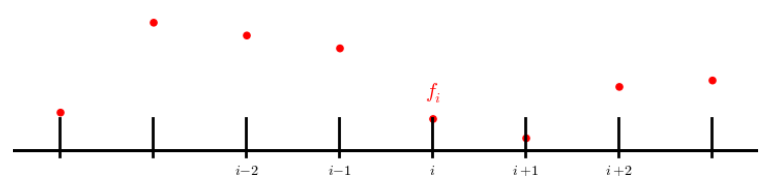
\includegraphics[width=30em]{13-22-29.png}

Sonlu hacim (FV) yönteminde durum biraz farklı; bir fonksiyonu belli
noktalarındaki noktasal değerlerle değil, belli aralıklar arasında kalan
değerlerinin averajı olarak temsil ediyoruz.

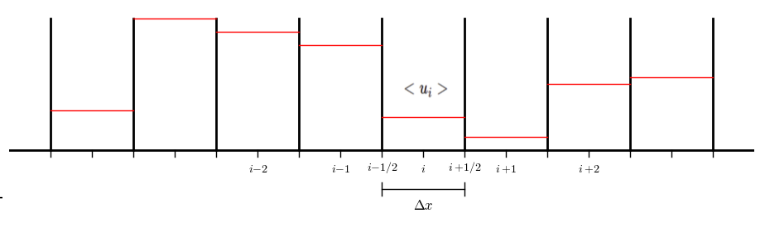
\includegraphics[width=30em]{13-22-34.png}

Farklı bir grafik

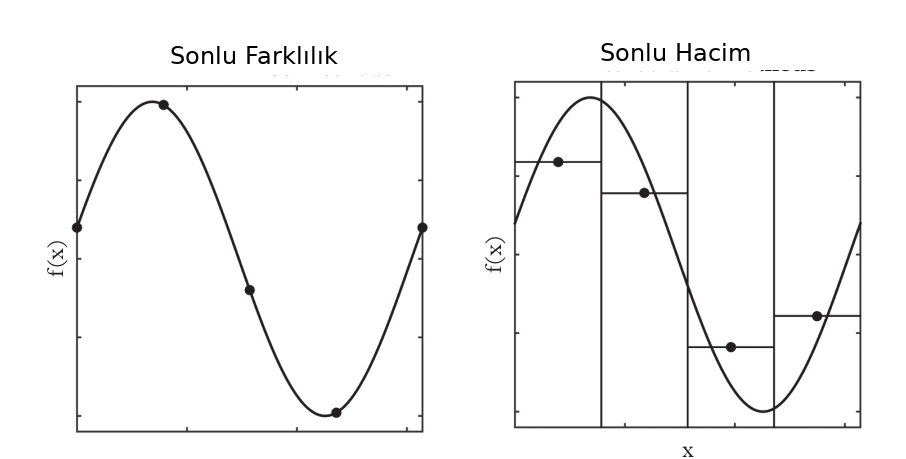
\includegraphics[width=30em]{13-16-00.png}

İki üstte görülen grafikte mesela $i$ ile $i+1$ noktası ortasındaki $i+1/2$
noktası ve $i$ ile $i-1$ noktası ortasındaki $i-1/2$ arasında kalan fonksiyonun
averajı alınacak, o zaman $< f_i >$ ya da $\overline{f}_i$

$$
\overline{f}_i = \frac{1}{\Delta x} \int _{x_{i-1/2}}^{x_{i+1/2}} f(x) \ud x
$$

Dikkat; $i-1,i-2$ değerleri $i$ referanslı olduğu için eksi içerikli, $i=4$
olsaydı onlar $3,2,..$ diye gidebilirdi. Ayrıca FD yönteminin aksine, indis
değerlerine tekabül eden $x_i,x_{i+1}$ değerleri herhangi bir yerde olabilir,
böylece eşit aralıklı olmayan ızgaralarla çalışmamız mümkün olur, bu FV
yönteminin kuvvetlerinden biri.

Notasyonda $f$ daha çok akış (flux) için kullanılır, karışıklık olmaması
için $u$ diyelim [2], $\Delta x$ için $h_x$,

$$
\overline{u}_i = 1/h_x \int_{x_{i-1/2}}^{x_{i+1/2}} u(x) \ud x
\mlabel{1}
$$

[3] yazısında muhafaza kanununun entegral formunu görmüştük,

$$
\int _{x_1}^{x_2} \rho(x,t_2) \ud x =
\int _{x_1}^{x_2} \rho(x,t_1) \ud x  +
\int_{t_1}^{t_2} \rho(x_1,t) v(x_1,t) \ud t -
\int_{t_1}^{t_2}  \rho(x_2,t) v(x_2,t) \ud t
$$

$f(\rho) = \rho(x,t) v(x,t)$ denebilir, ya da herhangi daha genel olarak $\rho$
yerine herhangi bir ölçüm $u$ için $f(u) = u(x,t) v(x,t)$, o zaman, ve
biraz yer değişim sonrası,

$$
\int_{x_1}^{x_2} u(x,t_2) \ud x -
\int_{x_1}^{x_2} u(x,t_1) \ud x  +
\int_{t_1}^{t_2} f(x_2,t) \ud t  -
\int_{t_1}^{t_2} f(x_1,t) \ud t = 0
$$

Bu formülü her sonlu hacim hücresi için kullanacağız. Zaman indisleri $t,t+1$
olacak, üstte $t_1,t_2$ yerine. Yer için $x_1,x_2$ yerine bir $j$ indisi
merkezli $x_{j-1/2}$ ve $x_{j+1/2}$. Devam edelim, $u(x_1,t_1)$ içinde
$x_{j-1/2}$ ve $t_l$ oluyor, (zaman $l$ indisi) ona da $u_{j-1}^l$
diyelim. $x_2$ yerine $x_{j+1/2}$, sonuncuda zamanın hala değişken olduğu durum
$u_{j+1}$ olsun. Eğer $x$ değişken ise, zaman indisi $t_2 = t_{l+1}$ için
$u^{l}$. Üstteki formülü bu notasyonla değiştirip istenen zaman ve yer
aralıklarına uygularsak,

$$
\int_{x_{j-1/2}}^{x_{j+1/2}} u^{l+1} \ud x -
\int_{x_{j-1/2}}^{x_{j+1/2}} u^{l} \ud x  +
\int_{t_l}^{t_{l+1}} f(u_{j+1/2}) \ud t  -
\int_{t_l}^{t_{l+1}} f(u_{j-1/2}) \ud t = 0
$$

Her şeyi $h_x$ ile bölelim,

$$
\frac{1}{h_x} \int_{x_{j-1/2}}^{x_{j+1/2}} u^{l+1} \ud x -
\frac{1}{h_x} \int_{x_{j-1/2}}^{x_{j+1/2}} u^{l} \ud x  +
\frac{1}{h_x} \int_{t_l}^{t_{l+1}} f(u_{j+1/2}) \ud t  -
\frac{1}{h_x} \int_{t_l}^{t_{l+1}} f(u_{j-1/2}) \ud t = 0
$$

Bu formülde (1)'de tanımlanan ortalama formunu görüyoruz, kısaltma amaçlı
$\overline{u}_{j,l}$ notasyonu oralarda kullanabiliriz,

$$
\overline{u}_{j,l+1} - \overline{u}_{j,l} + 
\frac{1}{h_x} \int_{t_l}^{t_{l+1}} f(u_{j+1/2}) \ud t  -
\frac{1}{h_x} \int_{t_l}^{t_{l+1}} f(u_{j-1/2}) \ud t = 0
$$

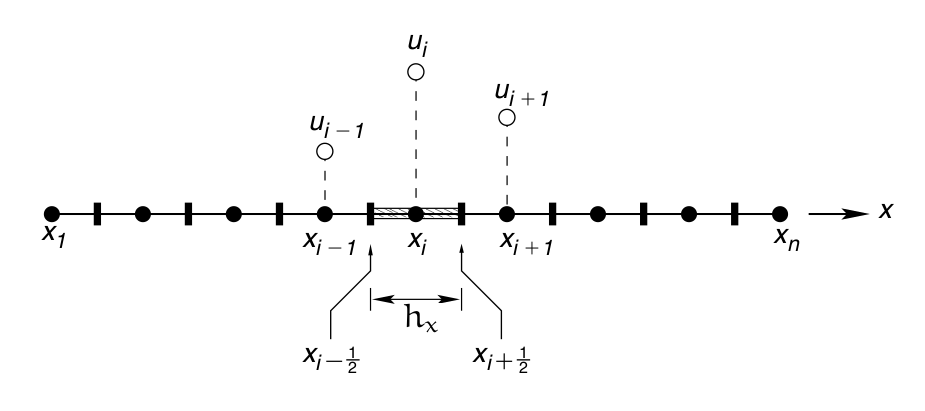
\includegraphics[width=20em]{12-20-00.png}
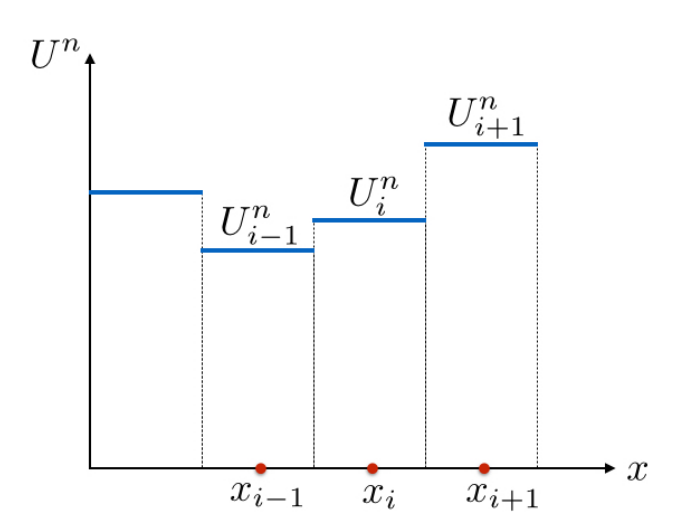
\includegraphics[width=20em]{12-19-02.png}




[devam edecek]
  
Kaynaklar

[1] Zingale, {\em PHY 604: Computational Methods in Physics and Astrophysics II}

[2] Kloeckner, {\em Numerical Methods for Partial Differential Equations CS555 / MATH555 / CSE510}
    \url{https://relate.cs.illinois.edu/course/cs555-s20/}

[3] Bayramlı, {\em Sonlu Hacim (Finite Volume) Yöntemi - 1}    

\end{document}
